\chapter*{AMとは}

AMラジオだFMラジオだ言っていますが、そういえばAMとかFMってなんでしょう。
AM、FMは電波の変調方式を示しています。つまり、電波に音を乗せる
方式のことです。音声信号を遠く離れたリスナーに届ける電波のことを
搬送波(はんそうは)と言います。この搬送波を変化させて音声信号を
載せるわけですが、振幅を変化させて音声信号を載せる方式を、
Amplitude Modulation、つまりAMと言います。
ちなみにFMはFrequency Modulationで周波数を変化させて音声信号を載せています。


\section*{AM変調の数学的理解}

周波数$f$の電波がアンテナに受信された時、その出力電圧を$V$とすると、
\begin{equation}
V = A\sin(2 \pi f t + \phi) = A\sin(\omega t + \phi)
\end{equation}
と書けます。ここで$A$を振幅、$\omega=2\pi f$を角振動数、$t$は時間、$\phi$を初期位相です。
この$A$を変化させて信号を乗せるのが、AMです。

この搬送波の周波数を$f_c$、振幅を$C$とすると、搬送波は
\begin{equation}
V_c = C\sin(2 \pi f_c t) = C\sin\omega_c t
\end{equation}
と書けます。初期位相が0なだけで、(1)式と全く同じ式です。

搬送波に乗せられる信号波$V_s$は、音声信号が単一の周波数$f_s$のみで構成されているとすると、振幅をSとすると、以下のように書けます。
\begin{equation}
V_s = S\sin(2 \pi f_s t) = S\sin\omega_s t \label{eq:AM_sig}
\end{equation}
\begin{figure}
\scalebox{0.2}{\rotatebox{-90}{\includegraphics{sig.ps}}}
\scalebox{0.2}{\rotatebox{-90}{\includegraphics{carr.ps}}}\\
\scalebox{0.2}{\rotatebox{-90}{\includegraphics{am.ps}}}
\scalebox{0.2}{\rotatebox{-90}{\includegraphics{spec.ps}}}
\caption{信号波(上段左)、搬送波(上段右)、AM変調波(下段左)、AM変調波のスペクトル(下段右)の例}
\end{figure}

この搬送波$V_c$が、$V_s$にAM変調されると、
\begin{eqnarray}
V_m &=& (V_s + C)\sin\omega_ct \label{eq:AM}\\ 
&=&(S\sin\omega_s t + C)\sin\omega_c t \nonumber \\
&=& V_s\sin\omega_s t \sin\omega_c t + C\sin\omega_c \nonumber \\
&=& \frac{V_s}{2}\{\sin(\omega_c + \omega_s)t + \sin(\omega_c - \omega_s)t\} + C\sin\omega_ct \label{eq:AM_exp}
\end{eqnarray}
となります。ここでは三角関数の公式$\sin\alpha\sin\beta=\frac{1}{2}\{\sin(\alpha+\beta)+\sin(\alpha-\beta)\}$を用いました。
%式(\ref{eq:AM_exp})を見ると、AM変調波は、$\omega_s \pm \omega_c$と、$\omega_c$の3つの周波数成分をもっていることがわかります。

図1に信号波、搬送波、変調波、周波数スペクトルの図を示します。
右上の搬送波に左上の信号波を変調すると、左下のように波の高さが
信号波に応じて変化しているのがわかります。これがAM変調波です。
右下の周波数スペクトルは、横軸が周波数のグラフで、
左下の図に含まれている周波数の分布を示しています。
3本の縦線が見えると思います。真ん中の長い線が、搬送波の周波数です。
残りの2本が信号波の成分です。
式(5)を見ると、$\sin$が3つ出てきていますね。
カッコの中身がそれぞれ違っています。1つは$\omega_c + \omega_s$、もうひとつは
$\omega_c - \omega_s$、最後に$\omega_c$。
つまり、搬送波の周波数を中心に、信号波の周波数分だけ離れた周波数の信号があることがわかります。

ここで、信号は$\omega_s$の単一の周波数成分しかもたないことを仮定しましたが、実際は複数の周波数成分をもっています。よって式(\ref{eq:AM})は、
\begin{eqnarray}
V_m &=&  (\sum_n s_n\sin\omega_n t + C)\sin\omega_c t \nonumber \\
&=& \sum_n a_n\sin\omega_n t \sin\omega_c t + C\sin\omega_c \nonumber \\
&=& \frac{1}{2}\sum_n{a_n\{\sin(\omega_c + \omega_n)t + \sin(\omega_c - \omega_n)t}\} + C\sin\omega_ct \nonumber
\end{eqnarray}
となります。これはシグマが付いているだけで、式(\ref{eq:AM_exp})と同じ形ですので、これ以降は、簡単のために信号波単一の周波数成分からなるものとしましょう。

\section*{IQ検波}
さて、本題のDSPを使った、AM変調波から信号波を取り出す原理を説明しましょう。
ちなみに、変調波から信号波を取り出すことを復調とか検波といいます。
AMラジオの検波の流れを示すために、DSPラジオIC Si4825-A10のデータシートにあるブロックダイアグラム図\ref{fig:block}を見てみましょう。


\begin{figure}
\scalebox{0.3}{\includegraphics{blockdiag.eps}}
\caption{DSPラジオIC SI4825-A10 のブロックダイアグラム}
\label{fig:block}
\end{figure}

アンテナから入力された信号は、ALC(Auto Level Control)回路で増幅率を制御された低ノイズアンプ(LNA:Low Noise Amp)で増幅することで入力レベルを一定にしています。
バツ印がマルで囲まれた記号は、Double Balanced Mixer (DBM)という回路です。
DBMは、入力信号と、基準信号を入力し、それらの
掛け算を出力する回路です。

基準信号は、AFC(Auto Frequency Control)で制御された、一定周波数の
発信機(マルにニョロの記号)から作られます。これを局部発振器と言います。

090と書かれたものは位相器で、波の位相を90度ずらした基準信号と
ずらさない基準信号を出力します。

さて、アンテナで受信された電波はアンプで増幅され、二分割されて
それぞれDBMの入力端子に入力されます。局部発振器でつくった基準信号は
位相器で位相を90度ずらしたもの、ずらさなかったものをそれぞれ
DBMに入力します。
位相を90度変化させた基準信号とアンテナからの入力を混合したものをQ成分、位相を変化させないものと混合したものをI成分と呼びます。
これらの二つの信号が、ADC(Analog/Disital Converter)でデジタル信号に変換されてDSPで数値計算処理されます。

局部発信器で作られた正弦波の周波数を$f_L$とし、振幅を$A_L$とすると、局部発信器の出力は
\begin{equation}
V_L = A_L \sin(2 \pi f_L t) = A_L \sin\omega_Lt
\end{equation}
となります。ここで$\omega_L = 2\pi f_L$です。DBMは、二つの入力端子の積を出力するので、I成分は、
\begin{eqnarray}
V_I &=& V_mA_L\sin(\omega_Lt + \frac{\pi}{2}) \nonumber\\
&=& V_mA_L\cos\omega_Lt \nonumber\\
&=& (V_s + C)\sin\omega_ct\cos\omega_Lt \nonumber\\
&=& \frac{V_s + C}{2}\{\sin(\omega_c + \omega_L)t + \sin(\omega_c - \omega_L)t\} \label{eq:AM_I}
\end{eqnarray}
となり、Q成分も同様に
\begin{eqnarray}
V_Q &=& V_mA_L\sin\omega_Lt \nonumber\\
&=& (V_s + C)\sin\omega_ct\sin\omega_Lt \nonumber\\
&=& \frac{V_s + C}{2}\{\cos(\omega_c + \omega_L)t - \cos(\omega_c - \omega_L)t \}\label{eq:AM_Q}
\end{eqnarray}
となります。ここでは、(4)式の$V_m=(V_s+C)\sin\omega_ct$を使いました。


\begin{figure}
\begin{minipage}{0.5\hsize}
\scalebox{0.2}{\rotatebox{-90}{\includegraphics{i.ps}}}
\caption{I成分}
\end{minipage}
\begin{minipage}{0.5\hsize}
\scalebox{0.2}{\rotatebox{-90}{\includegraphics{q.ps}}}
\caption{Q成分}
\end{minipage}
\end{figure}

\section*{数値計算によるAM変調波の検波}
さて、信号処理用のコンピュータであるDSPの中では何が行われているのでしょう。

(7)、(8)式を見てわかるように、$\sin$のカッコの中が$\omega_c+\omega_L$と
$\omega_c-\omega_L$の二種類があります。
両方に同じ信号の成分は含まれていますので、どちらか一方だけ使えば十分です。
一般に周波数が高くなると、ケーブルが理想的ではなくなったりして
回路を作成することが難しくなります。
よって周波数の高い$\omega_c + \omega_L$の成分を捨てて
$\omega_c \omega_L$の成分だけを使うことにします。
すると、I成分、Q成分は以下のようになります。
\begin{eqnarray}
V_I' &=& \frac{V_s+C}{2}\cos(\omega_c - \omega_L) \label{eq:AM_DSP_I}\\
V_Q' &=& \frac{V_s+C}{2}\sin(\omega_c - \omega_L) \label{eq:AM_DSP_Q}
\end{eqnarray}

準備ができたので、式(\ref{eq:AM_DSP_I})と式(\ref{eq:AM_DSP_Q})を二乗して足したものの平方根
を計算します。
\begin{eqnarray}
\sqrt{V_I'^2 + V_Q'^2} &=& \frac{V_s+C}{2}\sqrt{\cos^2(\omega_c - \omega_L)t + \sin^2(\omega_c - \omega_L)t }\\
&=& \frac{V_s}{2} + \frac{C}{2} 
\end{eqnarray}

なんとうことでしょう。$\sin$が消えて信号波の振幅$V_s$と、搬送波の振幅$C$の
足し算になったではありませんか。$C$は、DSPに入力される前にALCでほぼ一定
になっていますので、$C$は定数です。
DSPで高域フィルタ(High Pass Filter)の処理をすれば
直流成分$C$を除去することができます。
これではれて、信号波$V_s$だけ取り出すことができました。
これがIQ検波によるAM変調波復調の原理です。

最後に、GNU Rを使ってシミュレーションをしてみました。
結果を図\ref{fig:demodulation}に示します。
上部がガタガタして、高周波成分が残っているようです。今回のシミュレーションでは実装したフィルターがいまいちだったようです。
実際の回路やDSPの信号処理でも
素子の非線形性や、外乱などで回路やデジタル処理は理想的なものではありません。
(言い訳)
そこで高調波成分をLPFで除去すると、図\ref{fig:output}のようにきれいに信号波を、取り出すことができました。これは図1の上段左と同じ波形です!
あとは、スピーカーで音が出る程度にアンプで増幅してあげれば、AMラジオのできあがりです。
\begin{figure}
\begin{minipage}{0.5\hsize}
\scalebox{0.2}{\rotatebox{-90}{\includegraphics{demodulate.ps}}}
\caption{IQ検波された信号波}\label{fig:demodulation}
\end{minipage}
\begin{minipage}{0.5\hsize}
\scalebox{0.2}{\rotatebox{-90}{\includegraphics{out.ps}}}
\caption{LPF通過後の出力信号} \label{fig:output}
\end{minipage}
\end{figure}

シミュレーションに用いたソースコードを、Listing\ref{list:simulation}
に示しておきます。GNU Rのインストール方法、詳細は、\texttt{http://www.r-project.org}を参照してください。主要なLinuxディストリビューションではパッケージになっているので、そちらを使ったほうが楽にインストールできるでしょう。

\clearpage
\lstset{language=R,basicstyle=\ttfamily,numbers=left}
\lstinputlisting[caption=シミュレーションのソースコード,label=list:simulation]{sim.R}
